\documentclass{csse4400}

%\teachermodetrue

\usepackage{changepage}
\usepackage{enumitem}
\usepackage{languages}

\title{Architecture Modelling}
\author{Richard Thomas}

\date{\week{2}}
\begin{document}

\maketitle

\section{Before Practical}
Prior to attending your practical class,
\begin{itemize}[nosep]
    \item read \emph{at least} the \link{architectural views notes}{https://csse6400.uqcloud.net/schedule/\#week2} and this worksheet,
    \item review a modelling notation such as \link{UML}{https://www.uml-diagrams.org/} or \link{C4}{https://github.com/structurizr/dsl/blob/master/docs/language-reference.md},
    \item either install a modelling tool on your computer, or
    \item set up an account to use an online modelling tool, and
    \item explore the basics of the tool you plan to use.
\end{itemize}


\section{This Week}
Our goal is to get acquainted with a modelling notation and tool to be able to create diagrams to provide a visual representation of parts of a software architecture.
You will need to be able to produce diagrams representing parts of your architectural models throughout this course.


\section{Example System}
During this practical you will create a set of diagrams to describe the architecture of an on-line food delivery system (e.g. a simple \link{Uber Eats}{https://www.ubereats.com/au}).

Customers can search for restaurants that deliver to their address using a mobile or web application.
They can view restaurants on an interactive map to see their location.
They can select a restaurant to view its menu and select menu items to add to their order.
They can complete and pay for an order.
Customers can monitor the progress of their order through either the web or mobile apps.
Once their order has been collected for delivery, customers can track the location of the delivery agent.
Customers are notified by an alert in the app and a text message when the delivery agent is within 2 minutes of arriving.

Payment is handled through a payment gateway (e.g. PayPal, Stripe, ...).
When a customer completes an order, the system contacts the restaurant to submit the order.
The restaurant confirms acceptance of the order and gives an estimate of when it will be ready to be collected.
The system schedules a delivery agent to arrive at the restaurant by the estimated collection time.
Restaurants can update the system with a new estimated collection time.
This may cause the system to reschedule when the deliver agent will arrive or assign the delivery to a new agent.
The restaurant notifies the system when the order is ready to be collected.
The system notifies the delivery agent that the order is ready.

Delivery agents are people who deliver orders.
They have a mobile app that they use to register their location and availability to deliver orders.
When a delivery agent is allocated to collect an order from a restaurant, the app displays a map with a route to the restaurant from the agent's current location and estimated travel time.
When a delivery agent collects the order, they scan a QR code on the order to confirm they have collected the correct order.
Their mobile app then displays a map with a route to the delivery address.
The app sends the delivery agent's location to the system when they have moved 100 metres or they have been in one location for 2 minutes.

Restaurants interact with the system through either a web or mobile application.
They use their app to notify the system when they are able to accept orders and when they are not able to accept orders.
The app notifies the restaurant when an order has been placed.
The restaurant confirms acceptance of the order and enters an estimate of when the order will be ready.
The restaurant uses the app to indicate an order is ready and it prints out a delivery receipt with QR code that is attached to the order.

The system keeps track of customer browsing and order history.
It uses this data to make recommendations and special offers to customers.
Customers can view their past orders and reorder the same items or they may save orders as frequent orders.

Restaurants can view their accounts to see what orders have been placed and what income has been generated through the system.
The system pays restaurants by bank transfer on a weekly basis.

If a restaurant rejects an order, the system notifies the customer and refunds the purchase.
For simplicity, we will ignore details about how customers, delivery agents, and restaurants regsiter with the system.

\teacher{Have a class discussion to ensure that students have a reasonable idea of how to break the system into appropriate software systems,
               with some idea of key features of those systems.
               The intent is to get them to practice creating the models, not to design a good architecture.

               If the class is struggling to come up with a reasonable partitioning of the system, you can give them a basic partitioning.
               The text is intended to evoke ideas similar to the on-line store from the ``Architectural Views'' notes, so they have a structure to follow,
               but they do not have to follow that structure.
               The main point is that they should have a small number of software systems and deployment nodes.

               If there are different opinions of how to partition the system, let them go ahead and produce different models.
               If there is time, it would be good to compare the high-level diagrams of the different models and to discuss pros and cons of each approach.

               Leave details such as containers, components and interfaces until later in the practical.}


\section{Tools}
We do not support any specific tools in this course.
You may use any tools that you find easy to work with.
By this stage of your course and career, we expect that you have developed preferred ways to work.
We also expect that you can learn how to use tools from their support material.

The important thing is that you should use a modelling tool, not a drawing tool.
Many drawing tools provide UML templates, and some also support C4.
The issue with drawing tools is that they do not know what the elements of the diagram mean.
If the name of an operation in a class is changed in a drawing tool, you will need to manually change it wherever it is referenced in other diagrams
(e.g. in sequence diagrams).
A modelling tool will track the information that describes the model, so that a change to a model element in one place,
will be replicated wherever that element appears in other diagrams.

There are many tools that support UML.
In a commercial project using UML on a large system, the cost of professional UML tools is negligible and is quickly recovered by the automation they provide.
There are a number of free UML tools. Some to consider are \link{Astah}{https://astah.net/products/free-student-license/},
\link{ModelIO}{https://www.modelio.org/}, or \link{PlantUML}{https://plantuml.com/}.
\link{Visual Paradigm}{https://www.visual-paradigm.com/} is not as recommended, as their free cloud-based tool is only a drawing tool, and not a modelling tool.

\begin{description}
    \item[Astah]
        is a commercial product that supports visual modelling in many notations. They provide a free UML tool for students.
    \item[ModelIO] is an open source visual UML modelling tool.
    \item[PlantUML] Is an open source text-based descriptive language that generates UML diagrams.
        \link{PlantText}{https://www.planttext.com/} is an online tool supporting it.
    \item[Visual Paradigm] is a commercial product that supports visual modelling in many notations.
        They provide a simple free cloud-based drawing tool that supports UML and some limited aspects of C4, but it lacks full modelling support.
\end{description}

\noindent
There are fewer tools that support C4. Some to consider are \link{Structurizr}{https://www.structurizr.com/},
\link{C4-PlantUML}{https://github.com/plantuml-stdlib/C4-PlantUML}, \link{Archi}{https://www.archimatetool.com/},
\link{IcePanel}{https://icepanel.io/}, or \link{Gaphor}{https://gaphor.org/}.

\begin{description}
    \item[Structurizr]
        was developed by Simon Brown as a tool to support generating C4 diagrams from textual descriptions.
        UQ students may register for free access to the paid version of the \link{Structurizr Cloud Service}{https://structurizr.com/help/academic}.
        You must use your \texttt{student.uq.edu.au} or \texttt{uq.net.au} email address when you register to get free access.
        Structurizr is an \link{open source tool}{https://github.com/structurizr/}.
        You can use a domain specific language to describe a C4 model, or you can embed the details in Java or .Net code.
    \item[C4-PlantUML] which extends PlantUML to support C4.
    \item[Archi] is an open source visual modelling tool that
        \link{supports C4}{https://www.archimatetool.com/blog/2020/04/18/c4-model-architecture-viewpoint-and-archi-4-7/} and ArchiMate models.
    \item[IcePanel] is a cloud-based visual modelling tool that supports C4. There is a limited free license for the tool.
    \item[Gaphor] is an open source visual modelling tool that supports UML and C4.
\end{description}

\subsection{Textual vs Visual Modelling}
The tools described above include both graphical and textual modelling tools.
Graphical tools, such as Astah, ModelIO, Archi and Gaphor, allow you to create models by drawing them.
This approach is often preferred by \link{visually oriented learners}{https://vark-learn.com/strategies/visual-strategies/}.
Text-based tools, such as PlantUML and Structurizr, allow you to create models by providing a textual description of the model.
This approach is often preferred by \link{read/write oriented learners}{https://vark-learn.com/strategies/readwrite-strategies/}.

Despite preferences, there are situations where there are advantages of using a text-based modelling tool.
Being text, the model can be stored and versioned in a version control system (e.g. git).
For team projects, it is much easier for everyone to edit the model and ensure that you do not destory other team members' work.
It is also possible to build a tool pipeline that will generate diagrams and embed them into the project documentation.

Text-based modelling tools, such as Structurizr or PlantUML, use a
\link{domain specific language}{https://opensource.com/article/20/2/domain-specific-languages} (DSL) to describe the model.
These tools require that you learn the syntax and semantics of the DSL.
The following sources of information will help you learn the C4 DSL:
\begin{itemize}[nosep]
    \item \link{language reference manual}{https://github.com/structurizr/dsl/blob/master/docs/language-reference.md},
    \item \link{language examples}{https://github.com/structurizr/dsl/tree/master/docs/cookbook}, 
    \item \link{on-line editable examples}{https://structurizr.com/dsl}, and
    \item \link{off-line tool}{https://github.com/structurizr/cli/blob/master/docs/getting-started.md}.
\end{itemize}
You may find that the Sahara eCommerce C4 model is useful as an example of a number of features of the DSL.

The following sources of information will help you learn how to use the PlantUML DSL:
\begin{itemize}[nosep]
    \item \link{language reference manual}{https://plantuml.com/guide},
    \item \link{language overview with examples}{https://plantuml.com/}, and
    \item \link{on-line editable examples}{https://www.planttext.com/}.
\end{itemize}

\subsection{Example Diagrams}
You are able to download the UML and C4 models of the Sahara eCommerce example, from the course website.
The \link{UML model}{https://csse6400.uqcloud.net/resources/Sahara_eCommerce.asta}
was created using \link{Astah}{https://astah.net/products/free-student-license/}.
You may use this as an example of creating a model using a visual modelling tool.
There is a little more detail in the Astah model than what is shown in these notes.

The \link{C4 model}{https://csse6400.uqcloud.net/resources/c4_model.zip}
was created using the \link{Structurizr}{https://www.structurizr.com/} DSL
(\link{Domain Specific Language}{https://opensource.com/article/20/2/domain-specific-languages}).
You may use the C4 model as an example of creating a model using a textual description of the model (the DSL).


\teacher{It would be worth telling students the advantages of using a text-based DSL as a modelling language.
Specifically that the model can be stored in a version control system (e.g. git) and,
for team projects, this means it is much easier for everyone to edit the model.
It also means it is possible to build a tool pipeline that will generate diagrams and embed them into their documentation.

This then leads to discussing the advantage of using markdown for documentation.
It is easy for everyone in a team to edit the documentation,
and tools can automate the integration and generation of their complete set of documents.}


\newpage
\section{System Context}
Create a context diagram for the on-line food delivery system.
This may be a C4 system context diagram or a high-level business use case diagram with system boundaries
(\link{formally \textit{subjects} in UML}{https://www.uml-diagrams.org/use-case-subject.html}) \cite{uml}, and possibly packages.
Figures \ref{fig:c4_context} and \ref{fig:uml_context} are examples of these for the Sahara eCommerce example.

\begin{figure}[h!]
    \centering
    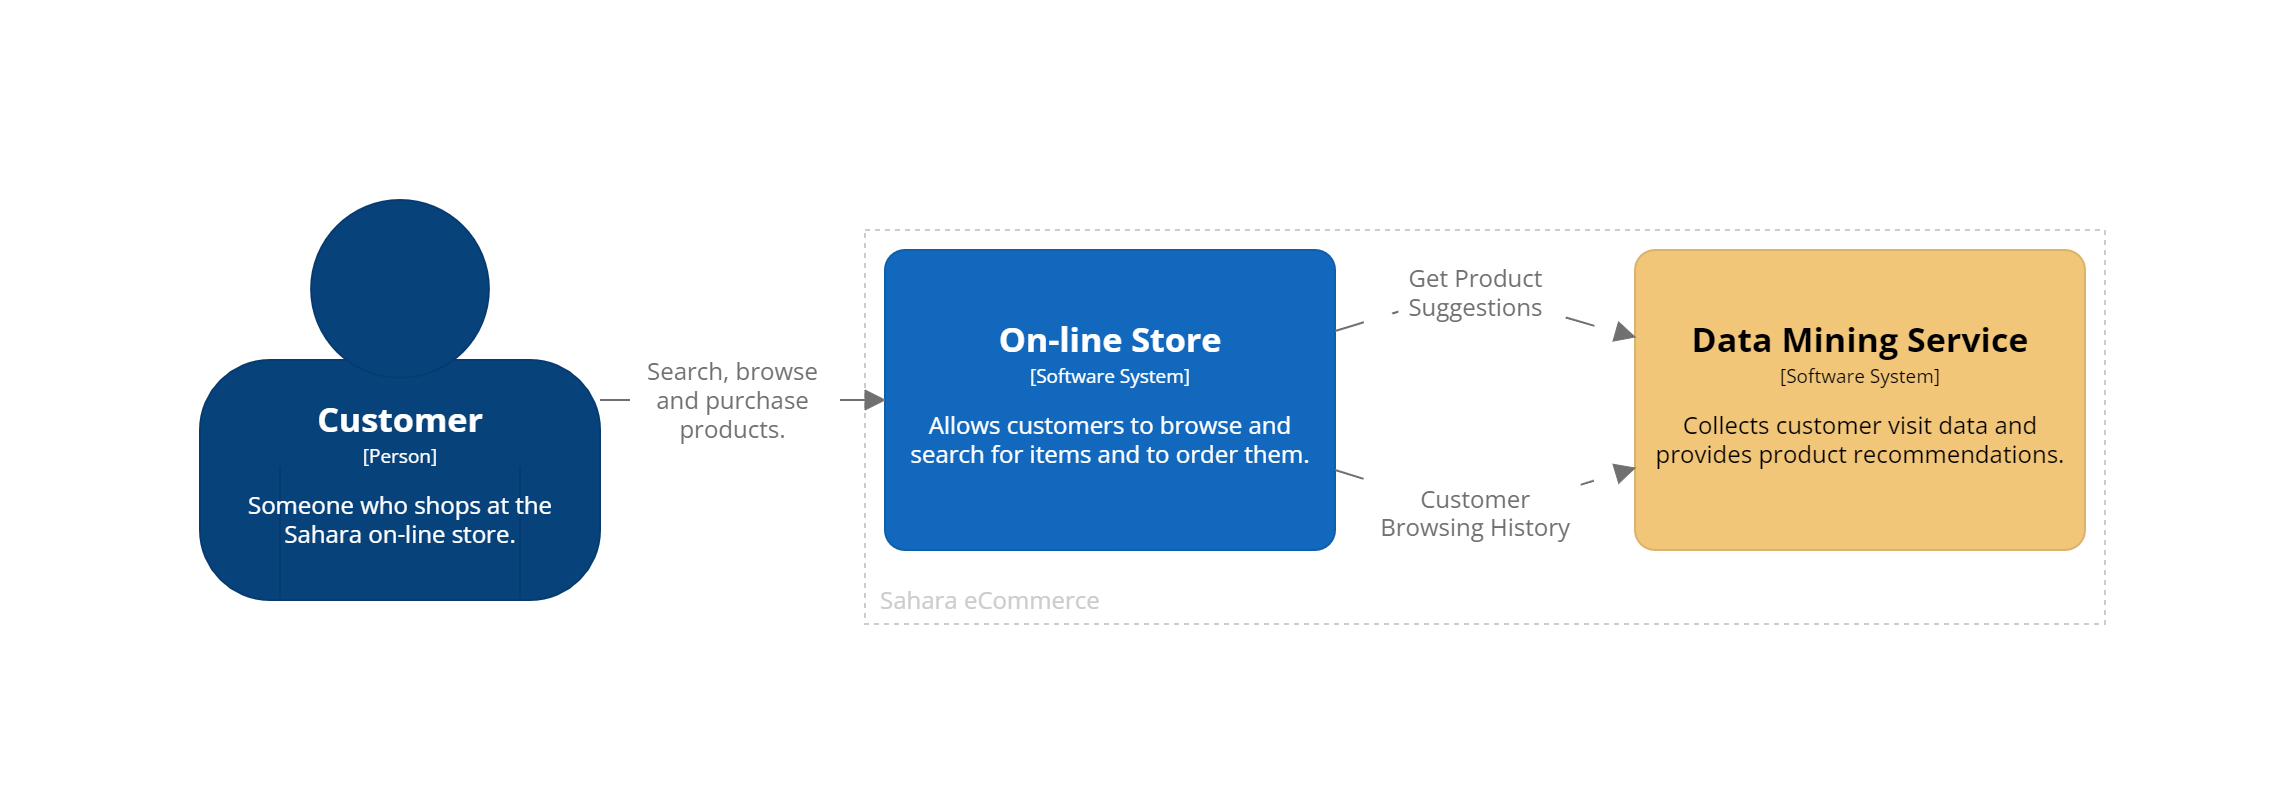
\includegraphics[trim=195 195 198 195,clip,width=0.9\textwidth]{../../notes/views/images/c4/context_diagram.png}
    \caption{C4 context diagram for the Saraha eCommerce on-line store.}
    \label{fig:c4_context}
\end{figure}

\begin{figure}[h!]
    \centering
    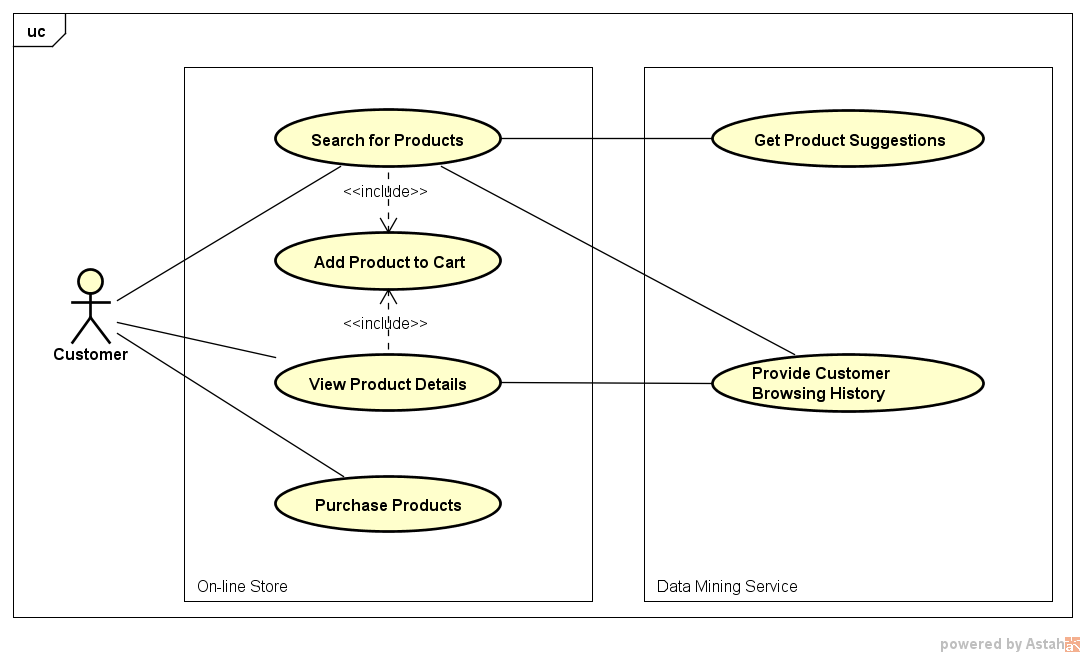
\includegraphics[trim=39 38 23 49,clip,width=0.8\textwidth]{images/uml-context.png}
    \caption{UML business use case diagram for the Saraha eCommerce on-line store.}
    \label{fig:uml_context}
\end{figure}

\teacher{Provide a quick summary of C4 context diagram and the UML business use case diagram, if some students seem a bit lost.
They weren't given the UML business use case diagram in the ``Architectural Views'' notes, as we used Bass et al's views, which do not include
context or use cases. You can compare the similarities between the diagrams.}


\newpage
\section{High-Level Software Architecture}
Create one or more high-level diagrams representing the core software architecture of the on-line food delivery system.
These may be C4 container diagrams or initial UML deployment diagrams.
The intent of these diagrams is to describe the overall structure of the system.
The focus is on the deployable software artefacts.
From a design perspective, you can decide \emph{how} these will be deployed onto computing infrastructure later.
Figures \ref{fig:c4_container_store} and \ref{fig:uml_deployment_software} are examples of these.

\begin{figure}[h!]
    \centering
    \begin{adjustwidth}{-5mm}{-5mm}
        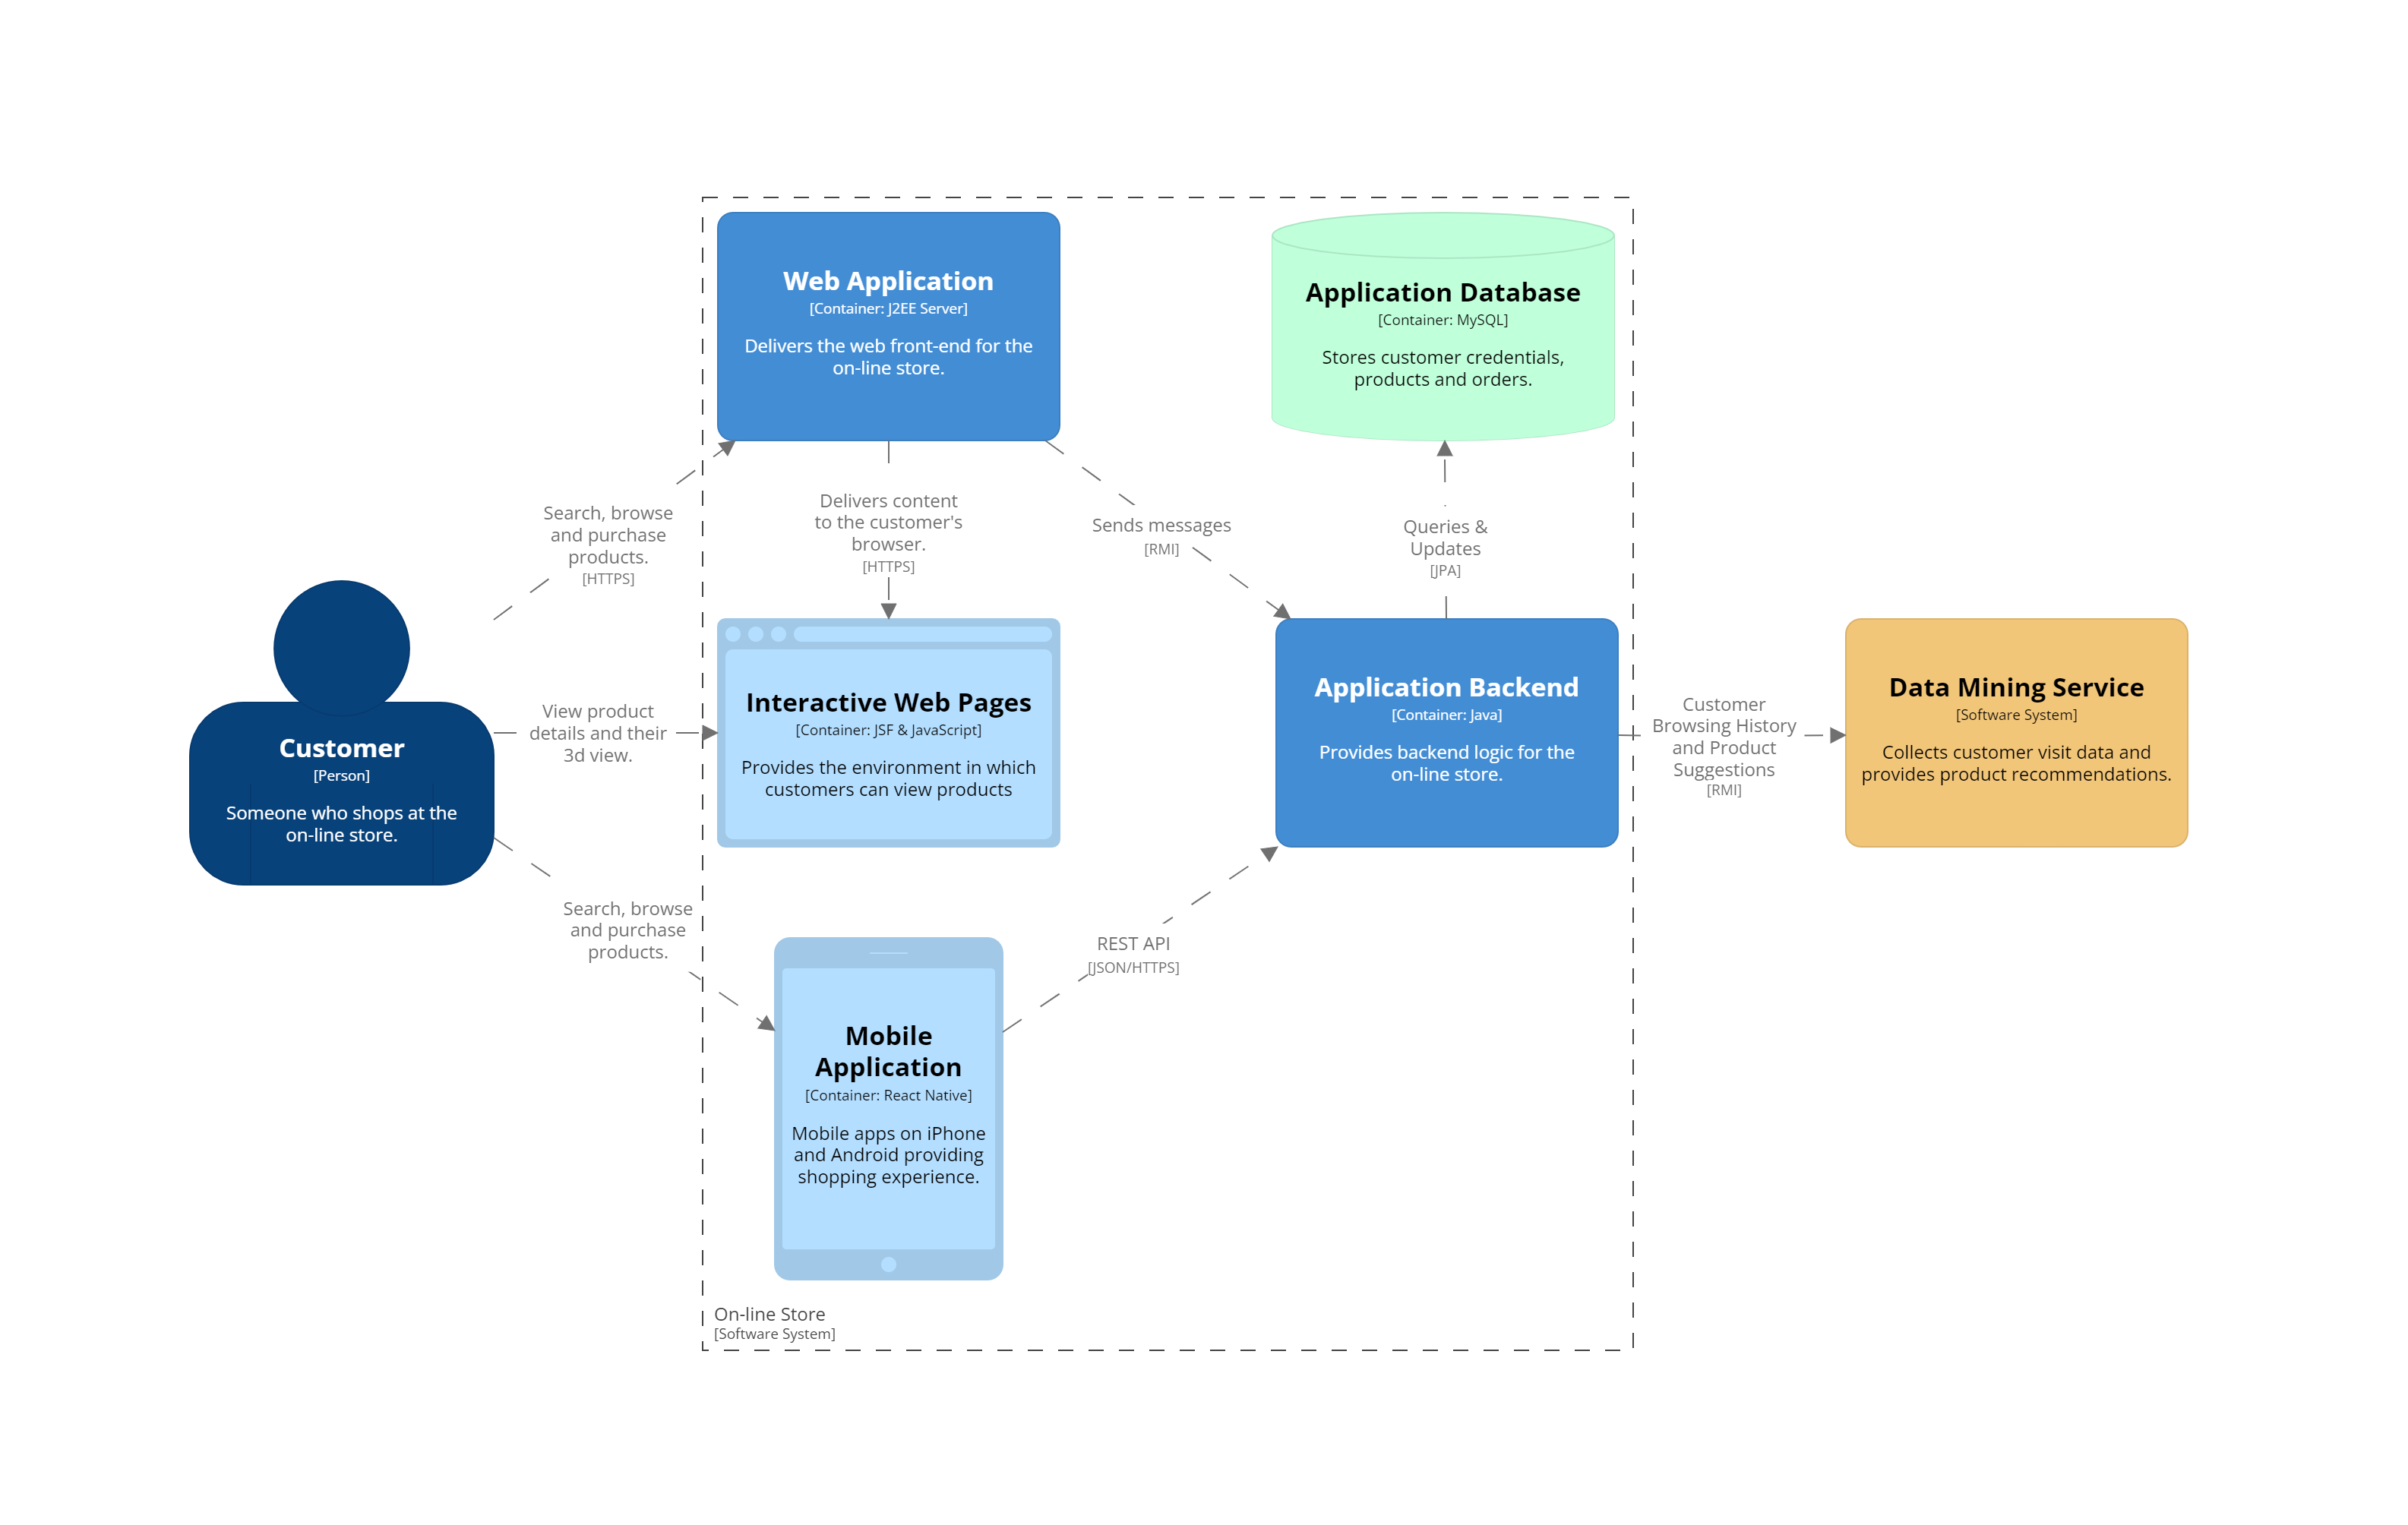
\includegraphics[trim=250 226 286 258,clip,width=0.92\paperwidth]{../../notes/views/images/c4/store_container_diagram.png}
    \end{adjustwidth}
    \caption{C4 container diagram for the on-line store software system.}
    \label{fig:c4_container_store}
\end{figure}

\begin{figure}[h!]
    \centering
    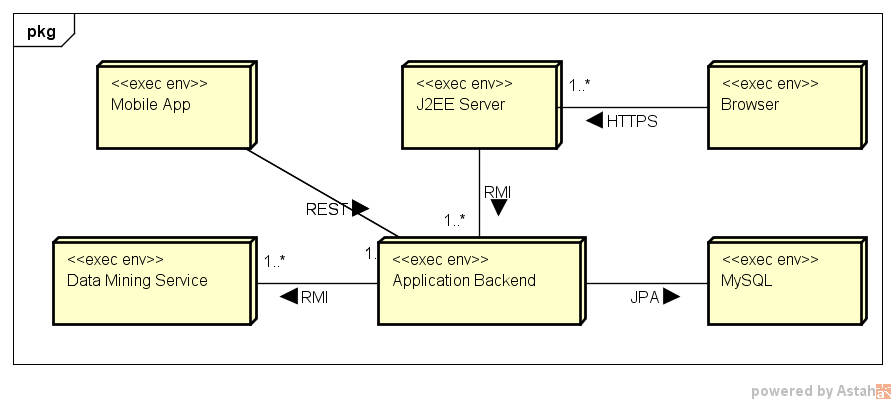
\includegraphics[trim=38 56 18 43,clip,width=0.8\textwidth]{images/software-deployment.png}
    \caption{UML deployment diagram for the software artefacts in the Saraha eCommerce system.}
    \label{fig:uml_deployment_software}
\end{figure}

\teacher{Provide a quick summary of C4 container diagram and the UML deployment diagram, if some students seem a bit lost.
They weren't given this UML deployment diagram of just the software artefacts in the ``Architectural Views'' notes.
You can compare the similarities between the diagrams.

Have a class discussion about possible deployable software artefacts for at least one software system.
The intent is to ensure they have identified a few artefacts that allows them to create at least one container or deployment diagram.

We are more interested in students getting experience using a modelling tool than we are with generating a complete set of architectural diagrams.
Once most students have at least one diagram, or at least seem to know how to create this type of diagram, move on to the next section.}


\newpage
\section{Components}
Create one or more C4 or UML component diagrams representing the internal structure of each deployable software artefact.
Given the time constraints of this session, you may wish to only produce one component diagram.
Figures \ref{fig:c4_component_appbackend} and \ref{fig:uml_component} are examples of these.

\begin{figure}[h!]
    \centering
    \begin{adjustwidth}{-5mm}{-5mm}
        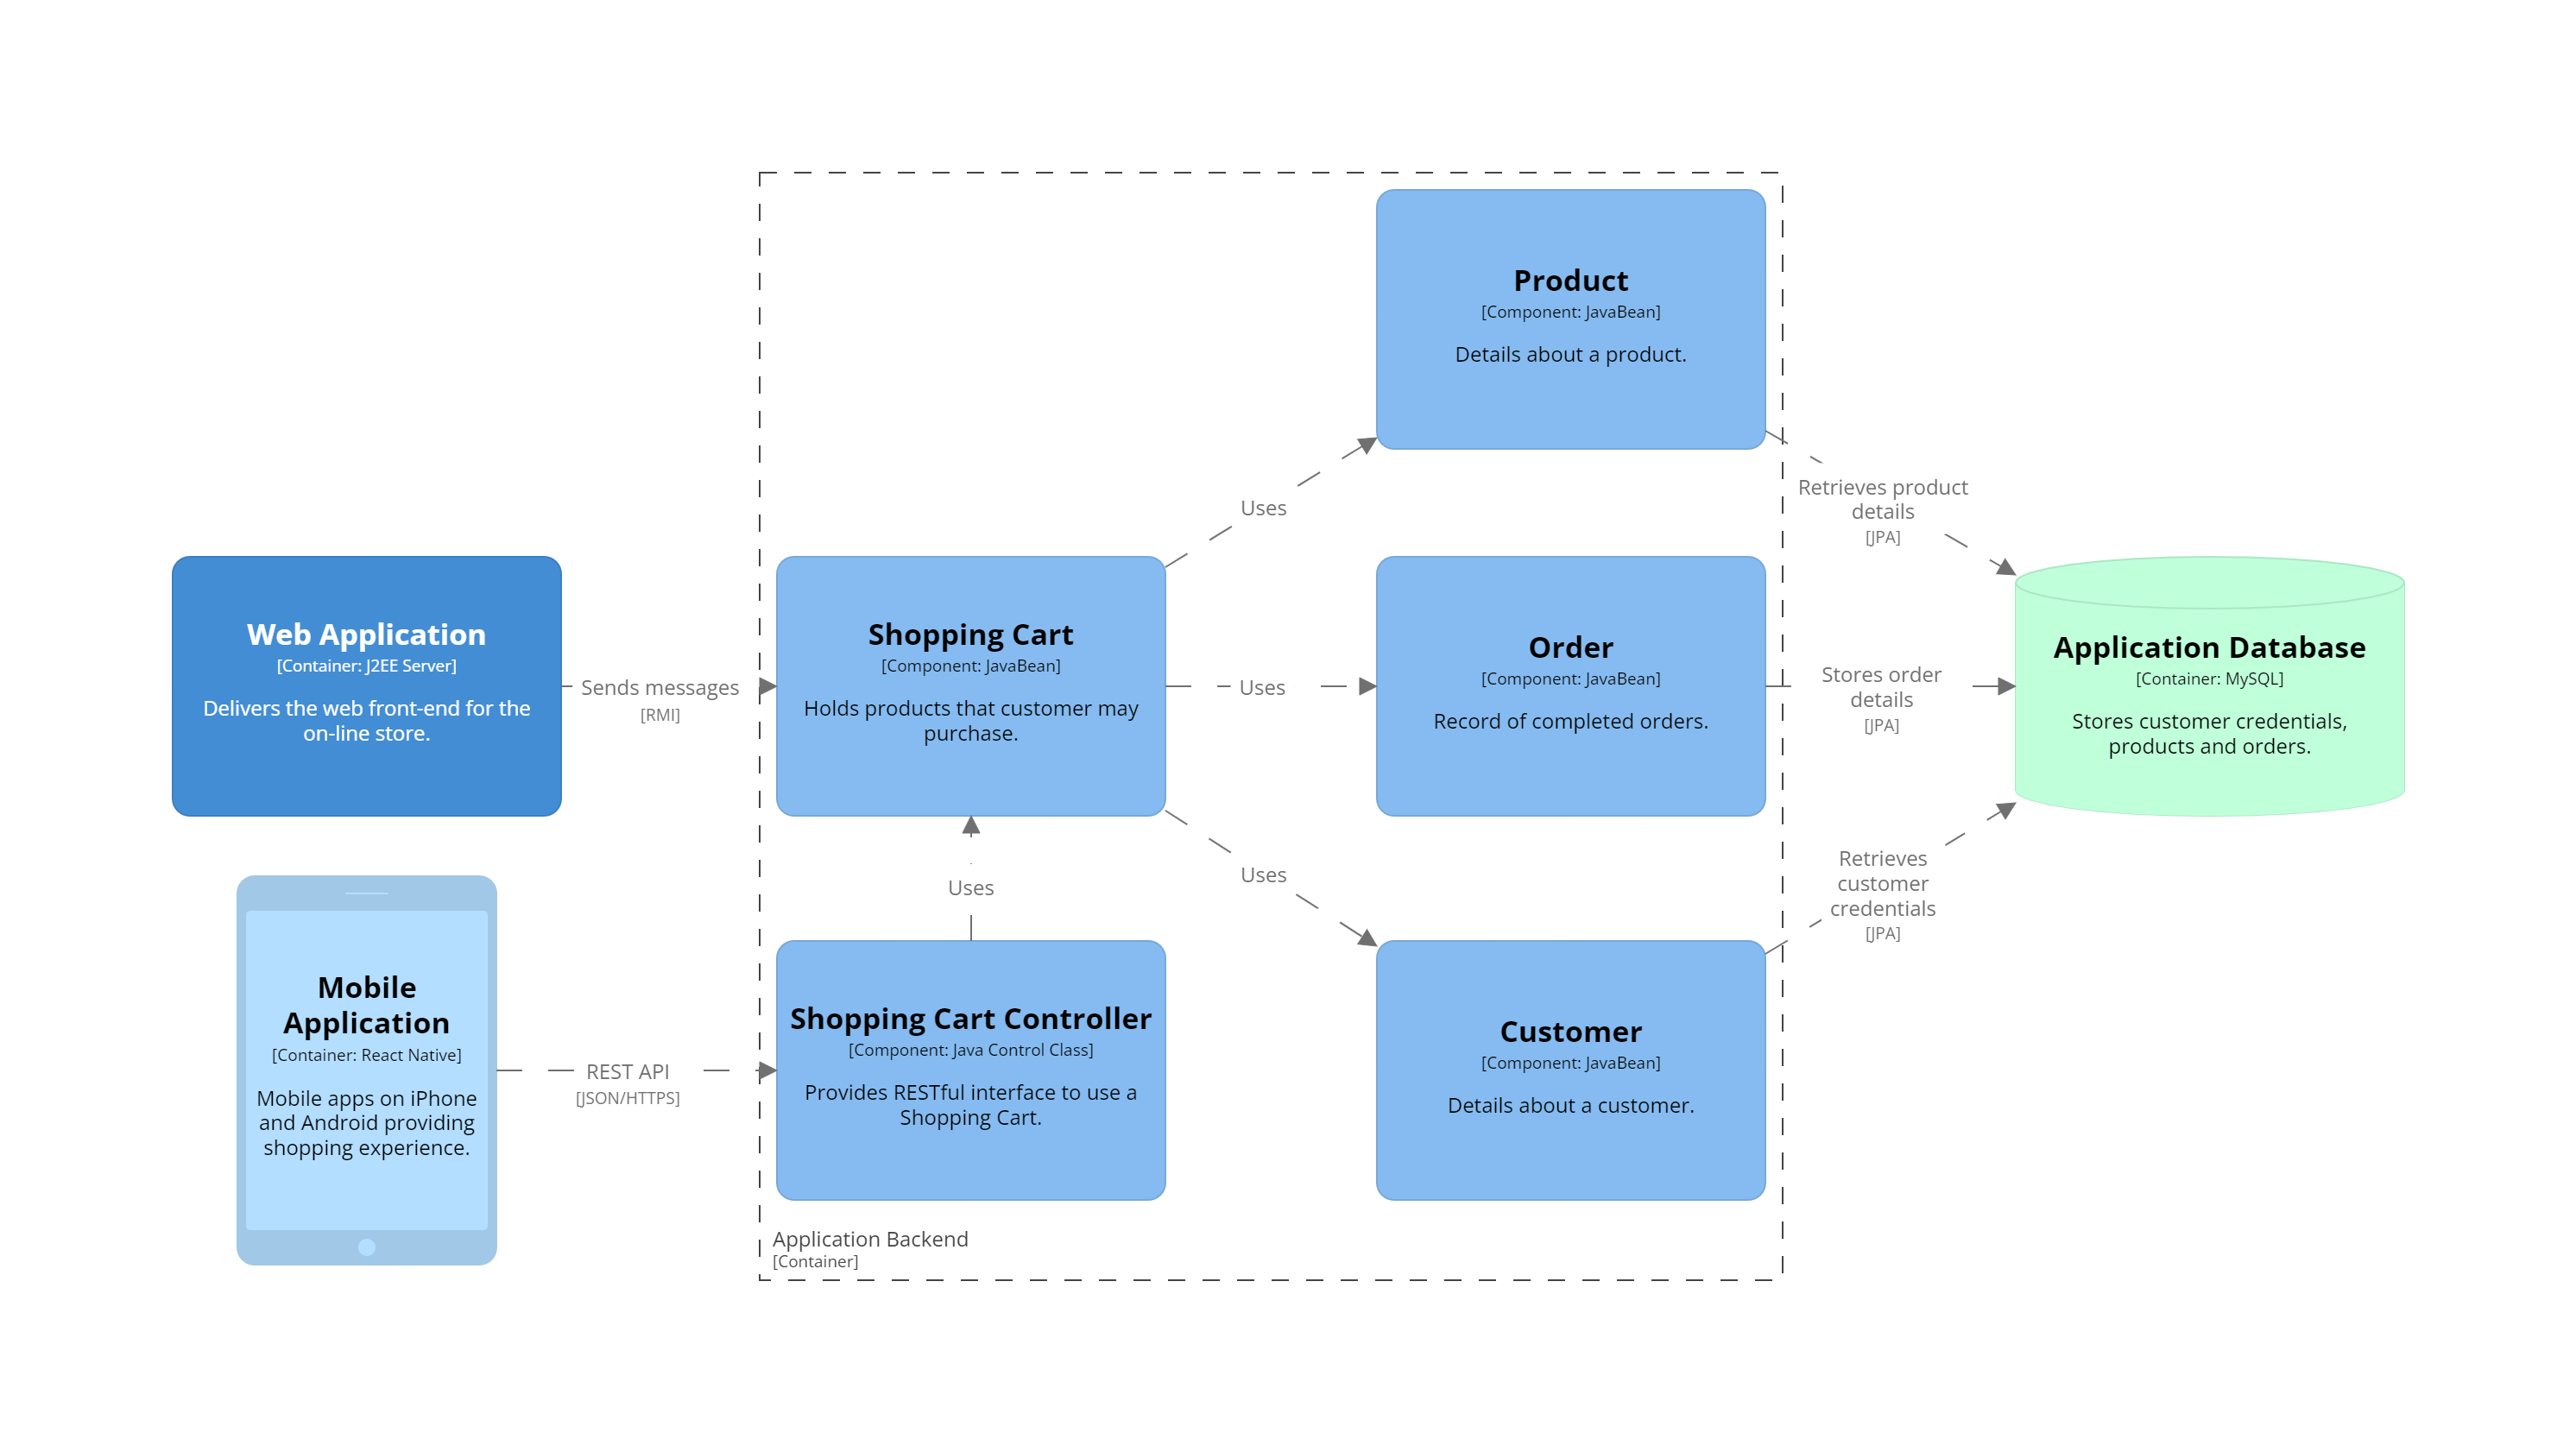
\includegraphics[trim=190 185 197 198,clip,width=0.92\paperwidth]{../../notes/views/images/c4/appbackend_component_diagram.png}
    \end{adjustwidth}
    \caption{C4 component diagram for the application backend container.}
    \label{fig:c4_component_appbackend}
\end{figure}

\begin{figure}[h!]
    \centering
    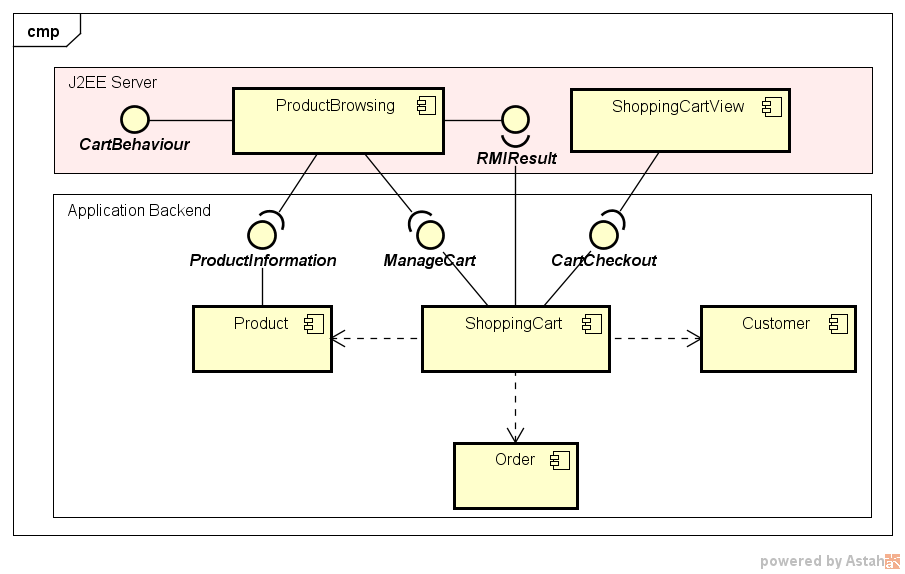
\includegraphics[trim=40 40 23 50,clip,width=0.72\textwidth]{images/uml-component.png}
    \caption{UML component diagram -- browsing for products and purchasing them.}
    \label{fig:uml_component}
\end{figure}

\noindent
C4 leaves details about interfaces to the code level, where they can be shown via a class diagram or other appropriate diagram or note.
UML does not require interfaces between components, but they are commonly used to provide a more rigorous description of the dependency between components.

\teacher{Provide a quick summary of C4 and UML component diagrams, if some students seem a bit lost.
Both of these are from the ``Architectural Views'' notes.
Mention that they should have seen them both before.

Describe the similarities and differences between the diagrams.
They reflect the characteristics and styles of the two modelling languages.
C4 focuses on the components within a container, and key communication with other containers.
Consequently, it includes both the web and mobile apps in the diagram, requiring a controller for the mobile app to interact with the cart.
UML modellers will often focus on the interfaces between components and their dependencies.
It only shows the web app and its interface connections to the application backend.

Have a class discussion about possible software components for at least one of the deployable artefacts.
The intent is to ensure they have identified a few components they can use to create a diagram.
For the purposes of this exercise, they don't need work out the details of the interfaces for UML.
They can just provide plausible names for the interfaces.
If you need them to get working, they can just show dependencies between components and ignore interfaces at this stage.

Again, once most students have at least one component diagram, or at least seem to know how to create one, move on to the next section.}


\newpage
\section{Component Behaviour}
Create one or more C4 dynamic diagrams, or UML sequence or communication diagrams,
providing examples of how components interact to deliver system functionality.
It is assumed that you are already familiar with UML class and sequence diagrams
(e.g. from \link{DECO2800}{https://my.uq.edu.au/programs-courses/course.html?course_code=DECO2800}
or \link{CSSE3200}{https://my.uq.edu.au/programs-courses/course.html?course_code=CSSE3200}).
Given time constraints, producing these diagrams may be left to be done in your own time.
Figures \ref{fig:c4_dynamic} and \ref{fig:uml_sequence_diagram} are examples of these.

\begin{figure}[h!]
    \centering
    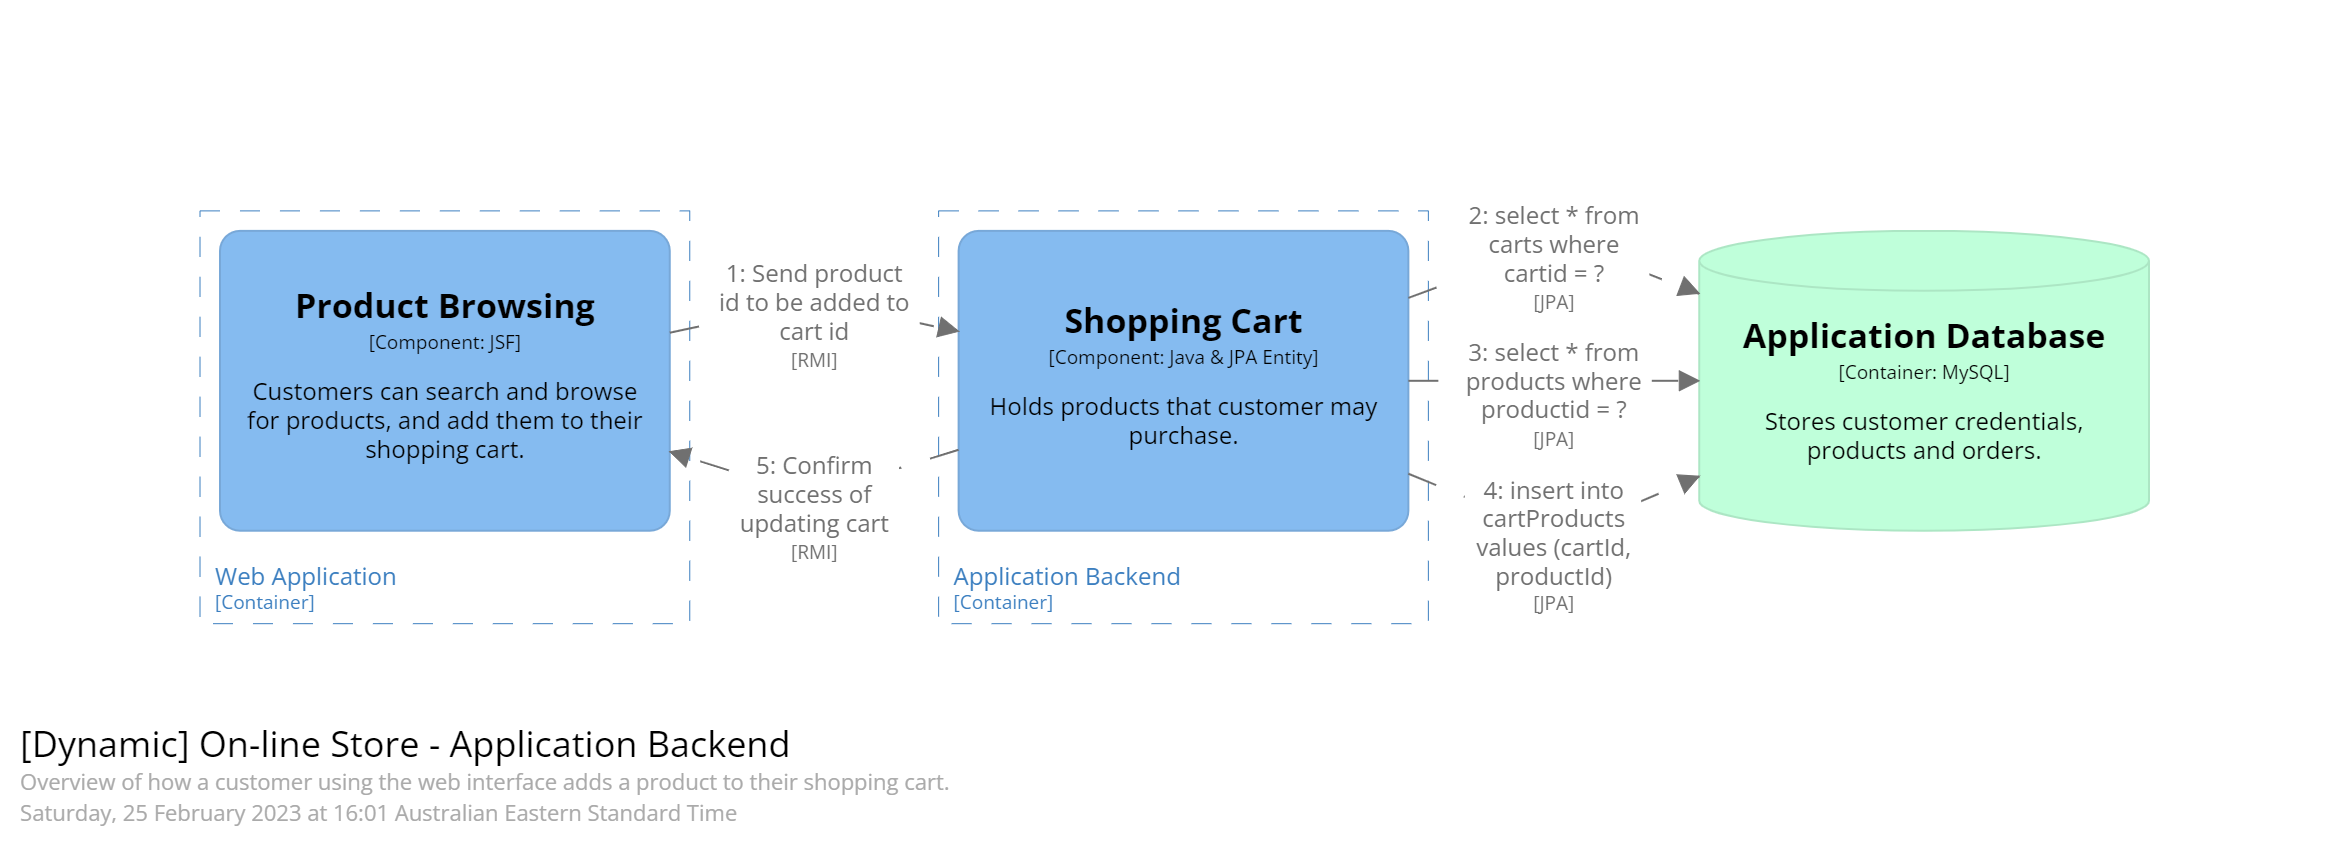
\includegraphics[trim=175 225 197 185,clip,width=\textwidth]{../../notes/views/images/c4/add_to_cart_dynamic_diagram.png}
    \caption{C4 dynamic diagram for adding a product to the customer's shopping cart.}
    \label{fig:c4_dynamic}
\end{figure}

\begin{figure}[h!]
    \centering
    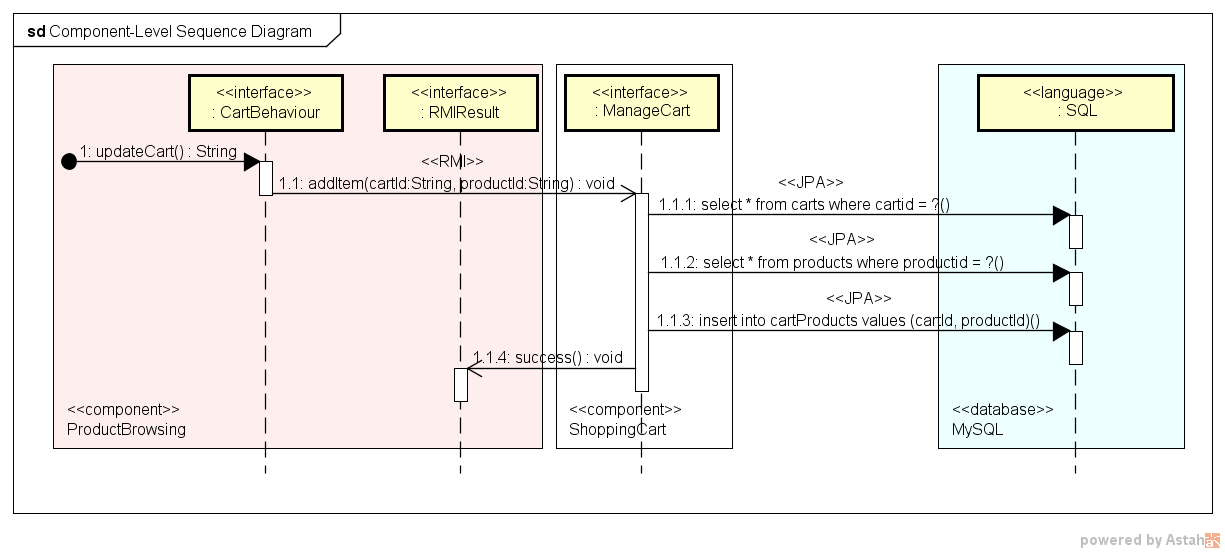
\includegraphics[trim=36 78 25 47,clip,width=\textwidth]{images/component-sequence.png}
    \caption{UML sequence diagram for adding a product to the customer's shopping cart.}
    \label{fig:uml_sequence_diagram}
\end{figure}

\noindent
If you use Astah, and many other UML modelling tools, you will encounter a constraint that they do not allow components to be used in sequence or communication diagrams.
Figure \ref{fig:uml_sequence_diagram} is the preferred approach to showing how components interact in a sequence or communication diagram.
Every component implements one or more interfaces, and instances that implement these interfaces are used in sequence or communication diagrams describing interactions between components.
Subjects can be used to group the instances that implement the interfaces together to show component boundaries.

Another option is to create redundant class diagrams to capture the operations used by each component.
Instances of these classes can be used to create sequence or communication diagrams describing interactions between components.
The classes are stereotyped as components to indicate that they correspond to components in the model.
This approach was shown in figure 4 in the ``Architectural Views'' notes.

Typically, when the database is only being used as a storage medium, it would not be shown in a sequence diagram.
Even a detailed sequence diagram would rarely show the SQL calls to a database.
This detail is only shown in this diagram to give an impression of what JPA does, assuming most of you are not familiar with it.

\teacher{Provide a quick summary of C4 dynamic diagrams and UML sequence diagrams.
Explain that the figure \ref{uml_sequence_diagram} is intentionally different to the component-level sequence diagram in the ``Architectural Views'' notes.

You will probably not have time to get students to create a dynamic or sequence diagram in the practical.}


\newpage
\section{System Deployment}
Create a C4 or UML deployment diagram describing the computing infrastructure on which the system will be deployed.
Show which software artefacts are deployed on which computing devices.
Figures \ref{fig:c4_deployment} and \ref{fig:uml_deployment} are examples of these.

\begin{figure}[h!]
    \centering
    \begin{adjustwidth}{-7.5mm}{-7.5mm}
        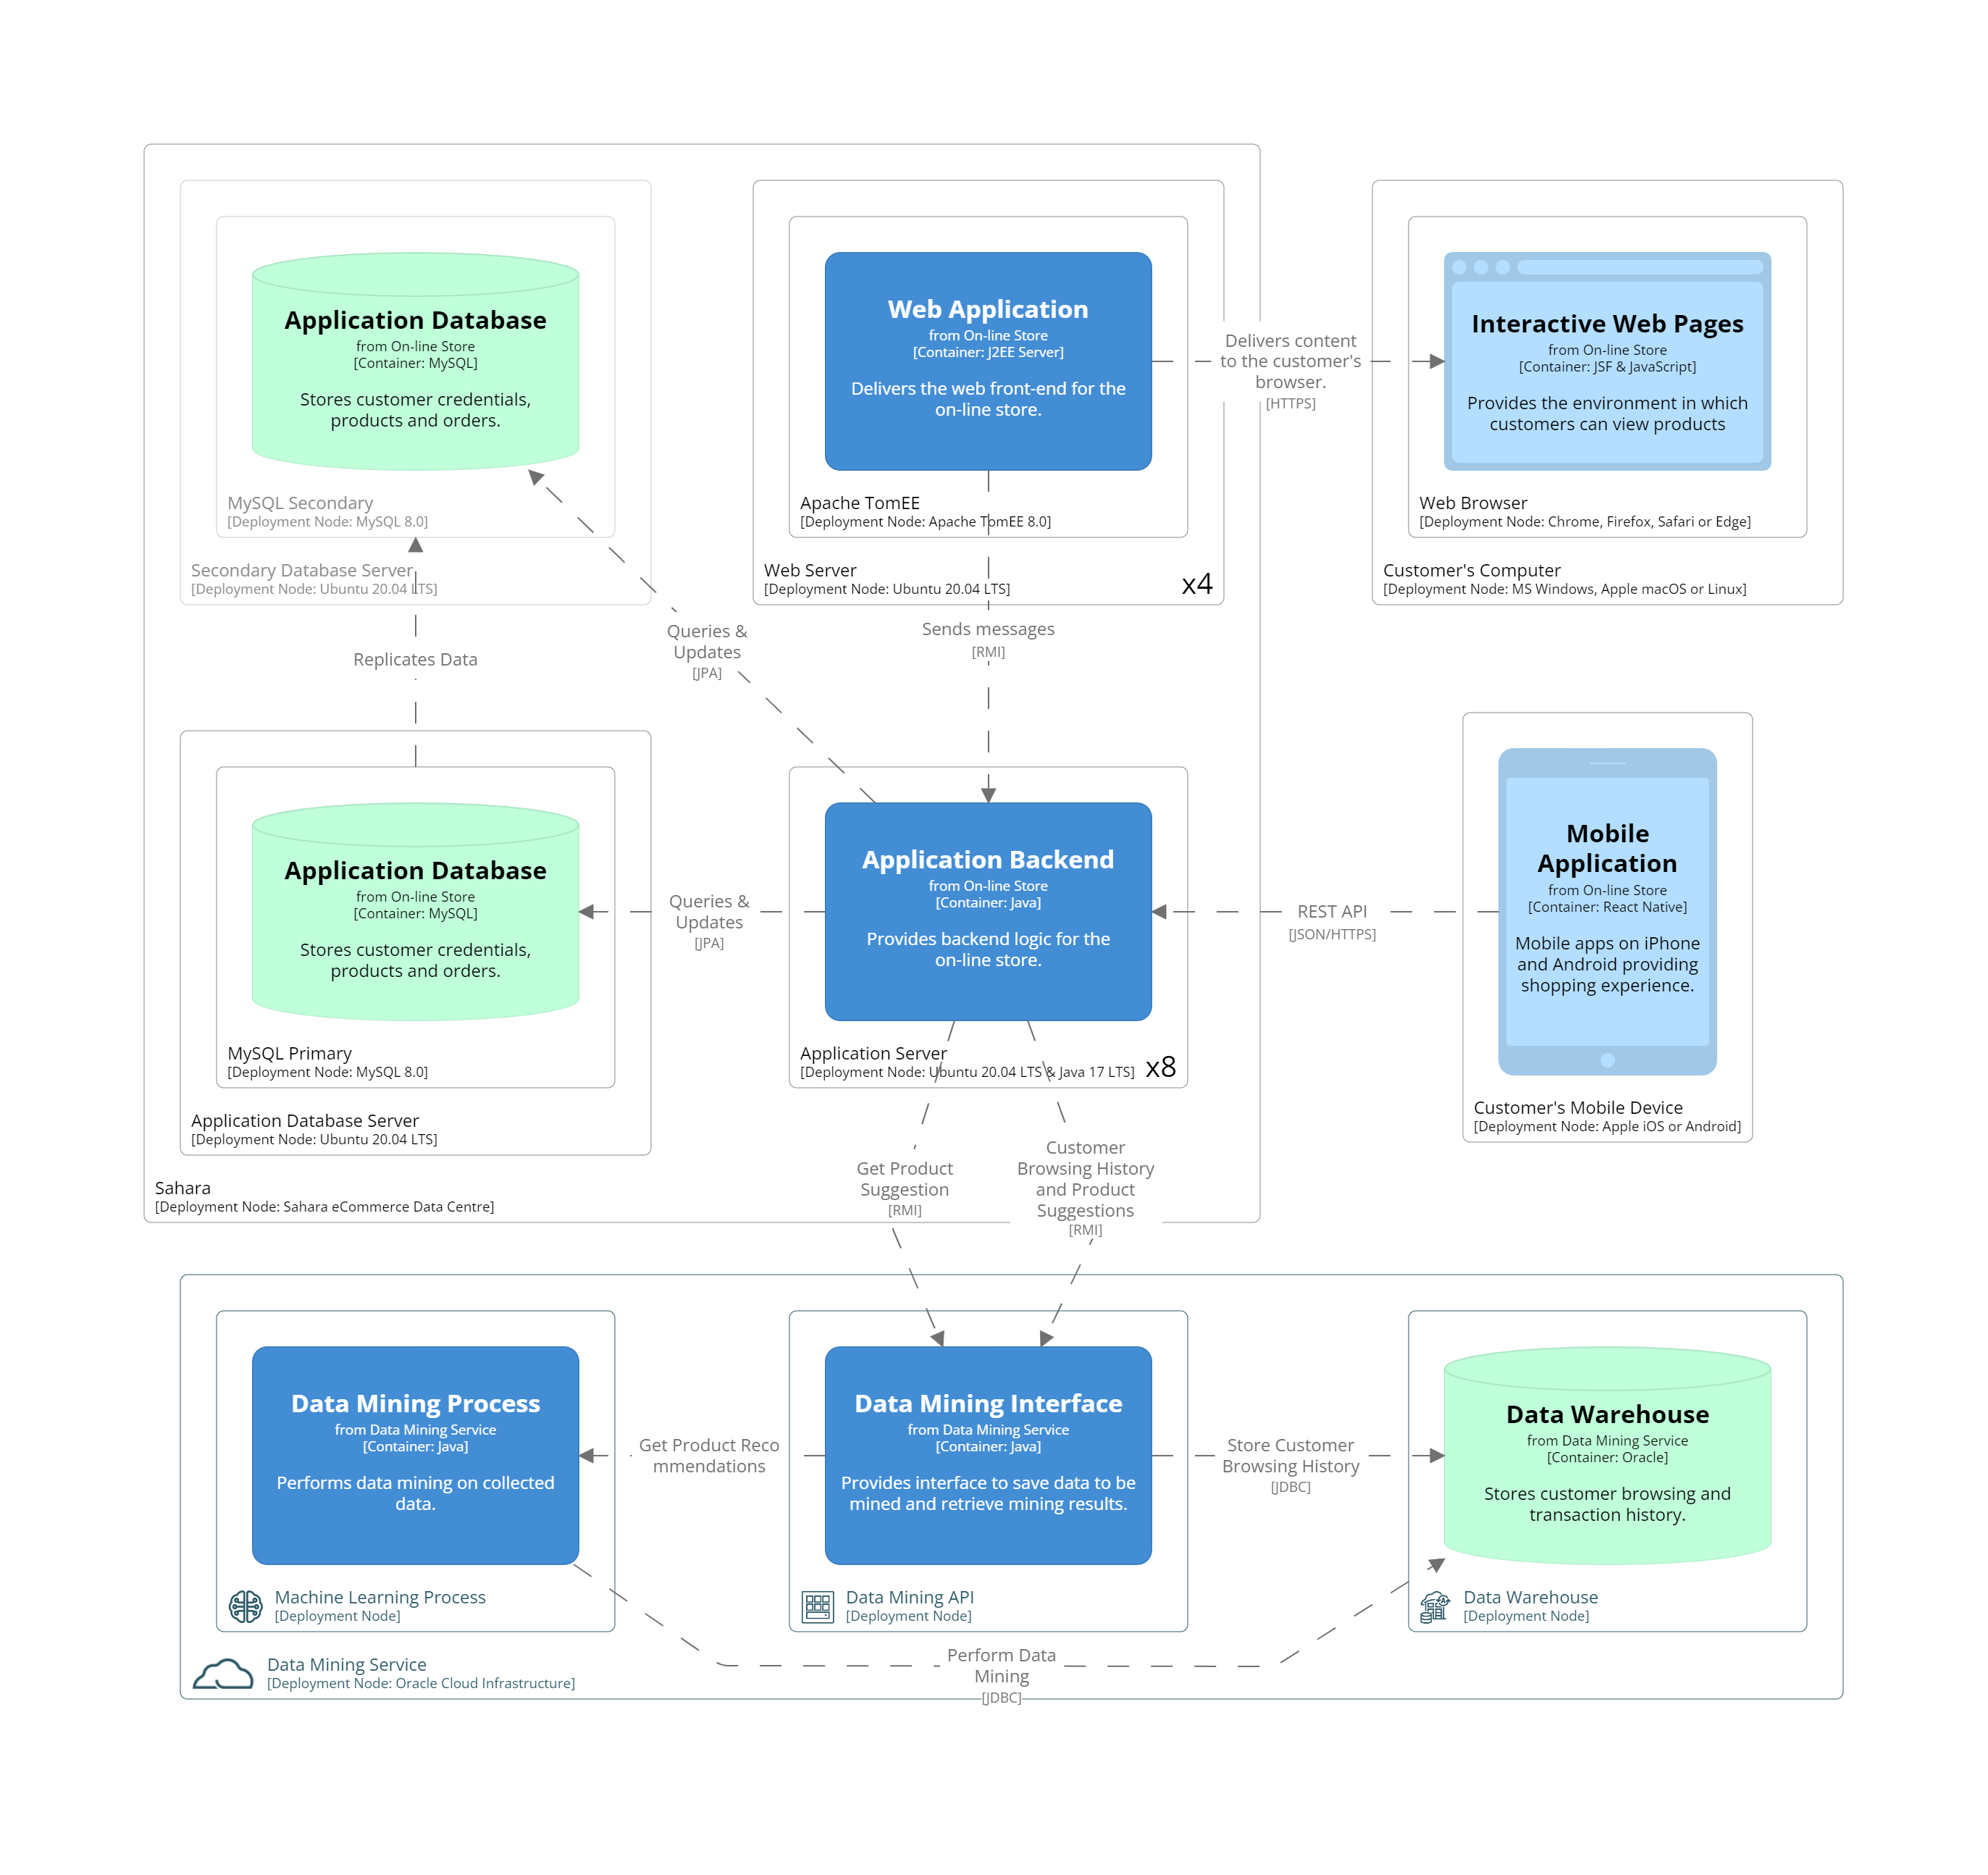
\includegraphics[trim=195 235 195 198,clip,width=0.95\paperwidth]{../../notes/views/images/c4/deployment_diagram.png}
    \end{adjustwidth}
    \caption{C4 deployment diagram for the Sahara eCommerce System.}
    \label{fig:c4_deployment}
\end{figure}

\begin{figure}[h!]
    \centering
    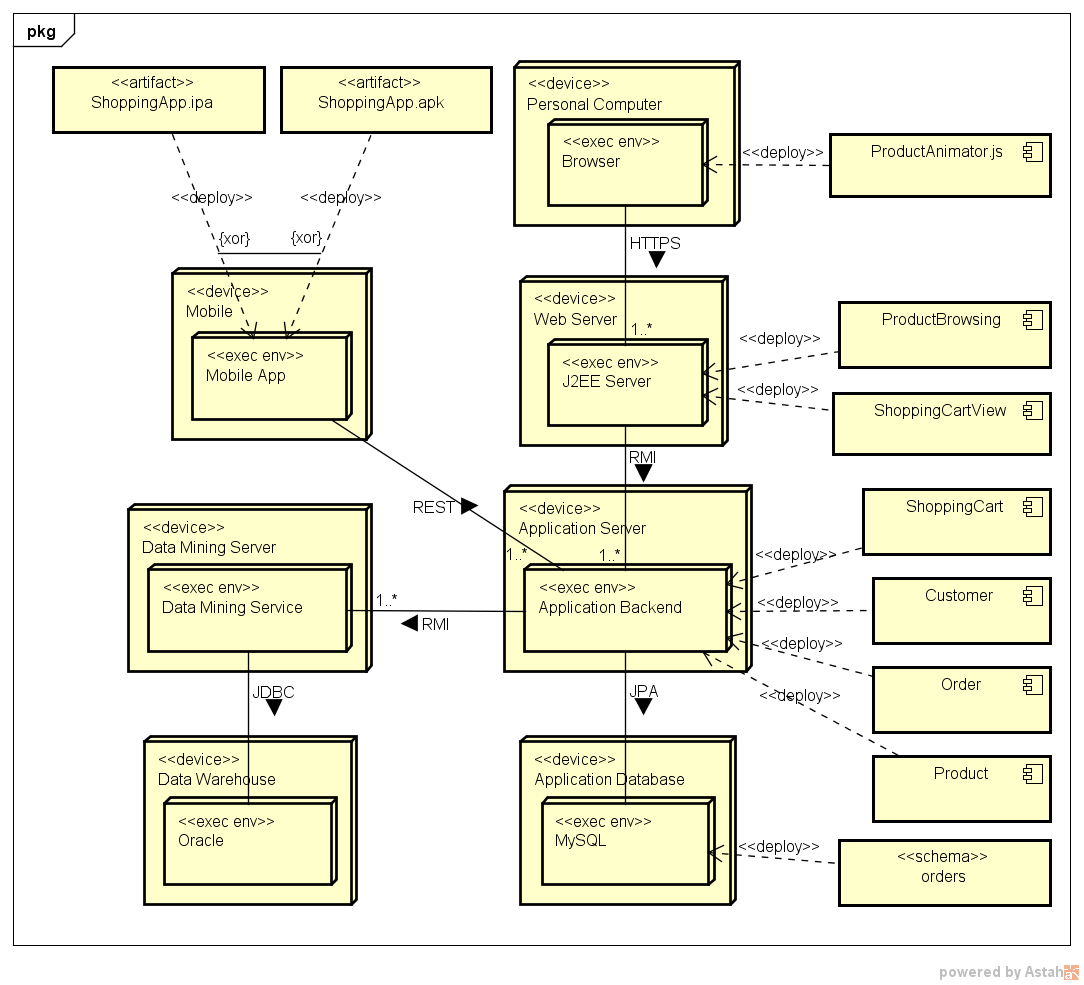
\includegraphics[trim=38 50 23 45,clip,width=0.95\textwidth]{images/uml-deployment.png}
    \caption{UML deployment diagram for the Sahara eCommerce system.}
    \label{fig:uml_deployment}
\end{figure}

\noindent
Figure \ref{fig:uml_deployment} shows the software artefacts from figure \ref{fig:uml_deployment_software},
as they will be deployed in the physical architecture.
Compared to the deployment diagram in the ``Architectural Views'' notes,
the iPhone and Android Phone devices have been simplified to being just a Mobile device.
The appropriate artifact is deployed to the Mobile device depending on its type.
The \texttt{\{xor\}} constraint is used to show that only one of those artifacts can be deployed as the Mobile App on a Mobile device.

\teacher{Provide a quick summary of C4 and UML deployment diagrams, if some students seem a bit lost.
The UML deployment diagram is modified from what is in the ``Architectural Views'' notes, as is mentioned above.
You may want to summarise the differences.

Have a class discussion about how the software artefacts for the on-line food delivery could be deployed.
Some deployment nodes should be obvious from the description, but there are some options for the company's internal systems.
You can decide if you want them to think about physical hardware or cloud infrastructure.}


\filbreak\newpage
\section{Detailed Design}
Create one or more class diagrams, with accompanying sequence or dyanmic diagrams, describing how components will be implemented.
Do not create diagrams for the complete system, rather create a few that highlight some interesting aspects of your proposed design.
Given time constraints, producing these diagrams may be left to be done in your own time.
Figures \ref{fig:uml_class} and \ref{fig:uml_detailed_sequence} are examples of these.

\begin{figure}[h]
    \centering
    \begin{adjustwidth}{-10.5mm}{-11mm}
        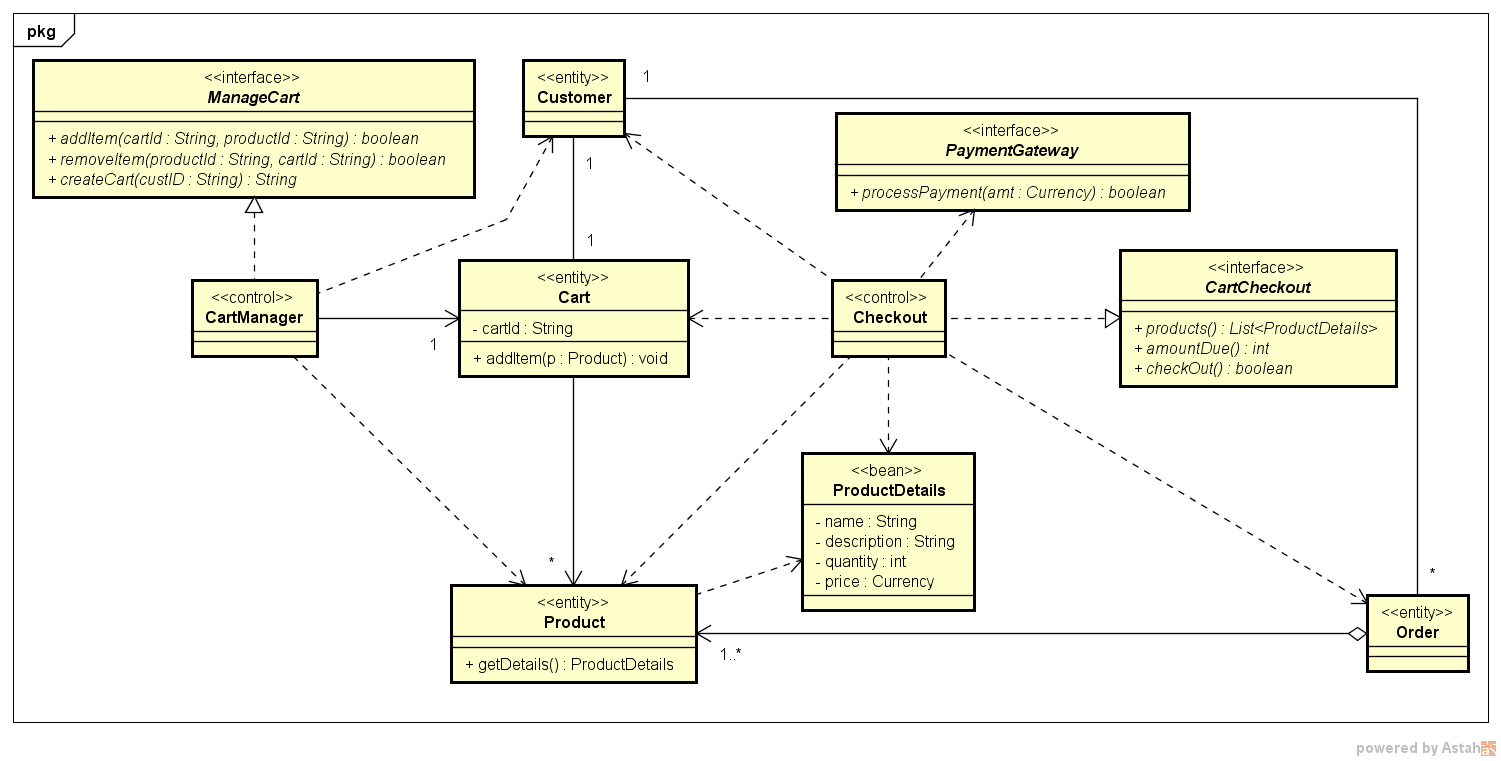
\includegraphics[trim=22 45 22 44,clip,width=0.98\paperwidth]{../../notes/views/images/uml/shopping_cart_class_diagram.png}
    \end{adjustwidth}
    \caption{UML class diagram for part of the shopping cart package in the class model.}
    \label{fig:uml_class}
\end{figure}

\begin{figure}[h!]
    \centering
    \begin{adjustwidth}{-11mm}{-11mm}
        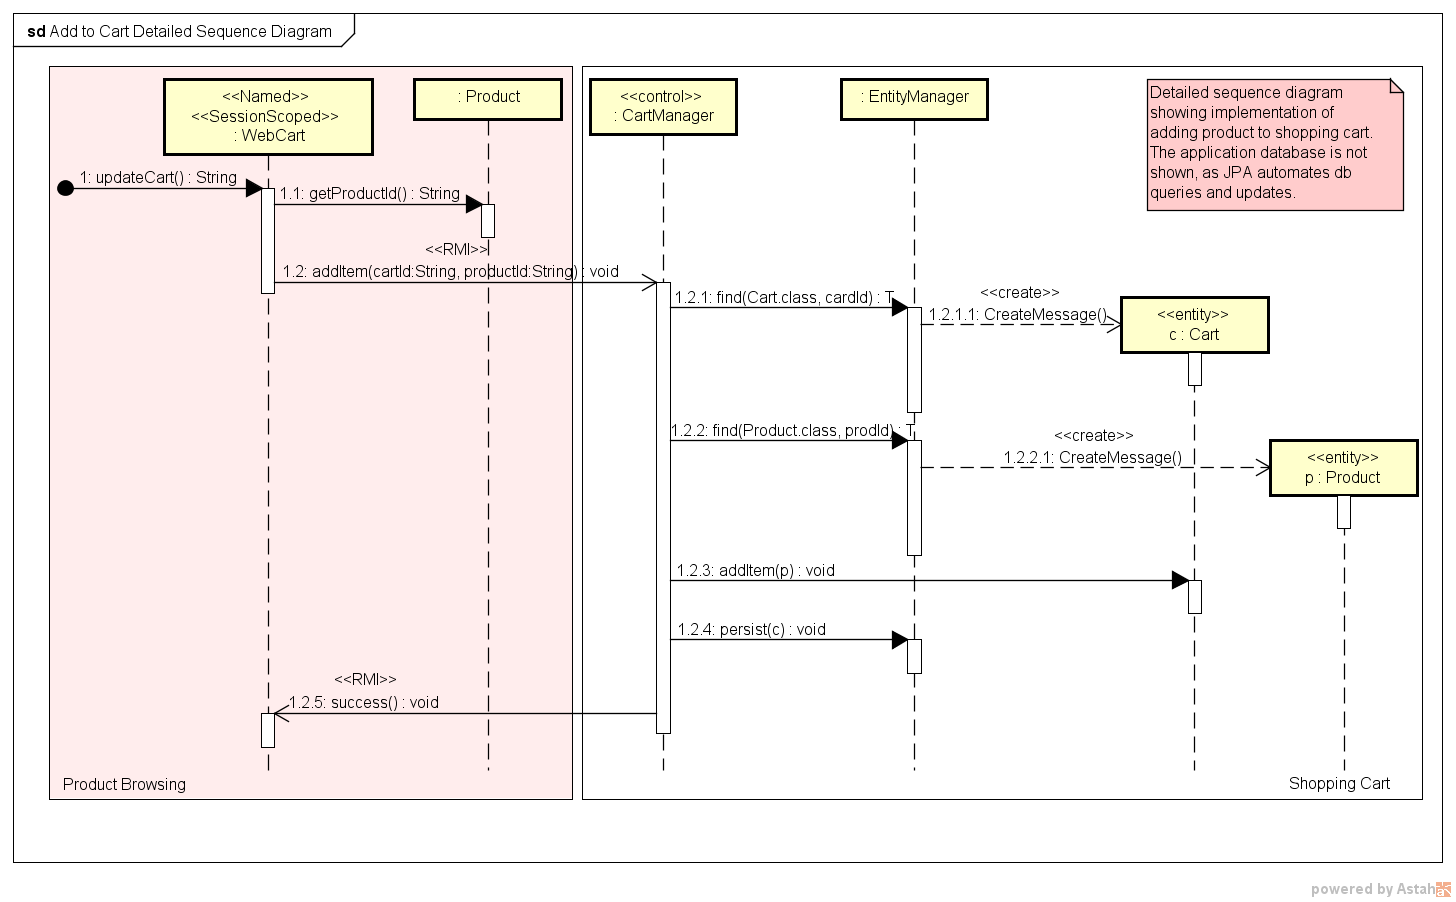
\includegraphics[trim=35 70 31 49,clip,width=0.98\paperwidth]{../../notes/views/images/uml/detailed_sequence_diagram.png}
    \end{adjustwidth}
    \caption{Detailed UML sequence diagram showing the implementation of customer adding a product to their shopping cart.}
    \label{fig:uml_detailed_sequence}
\end{figure}

\filbreak
Subjects are used in figure \ref{fig:uml_detailed_sequence} to show software system boundaries.

\teacher{Provide a quick summary of UML class diagrams, if some students are not familiar with them.
These are both from the ``Architectural Views'' notes.

You will probably not have time to get students to create a class diagram in the practical.}


%\todo{Get Brae to integrate plantuml diagrams better}
%\includegraphics[width=0.9\textwidth]{images/examplec4}


\newpage
\section{Further Work}
Continue working on your diagrams to produce a complete model of the software architecture for the on-line food delivery system.
Share your ideas, diagrams, and model source on Slack.


\bibliographystyle{ieeetr}
\bibliography{refs}

\end{document}